%%%%%%%%%%%%%%%%%%%%%%%%%%%%%%%%%%%%%%%%%%%%%%%%%%%%%%%%%%%%%%%%%%%%%%%%%%%%%%%%
%2345678901234567890123456789012345678901234567890123456789012345678901234567890
%        1         2         3         4         5         6         7         8

\documentclass[letterpaper, 10 pt, conference]{ieeeconf}  % Comment this line out
                                                          % if you need a4paper
%\documentclass[a4paper, 10pt, conference]{ieeeconf}      % Use this line for a4
                                                          % paper

\IEEEoverridecommandlockouts                              % This command is only
                                                          % needed if you want to
                                                          % use the \thanks command
\overrideIEEEmargins
% See the \addtolength command later in the file to balance the column lengths
% on the last page of the document



% The following packages can be found on http:\\www.ctan.org
%\usepackage{graphics} % for pdf, bitmapped graphics files
%\usepackage{epsfig} % for postscript graphics files
%\usepackage{mathptmx} % assumes new font selection scheme installed
%\usepackage{times} % assumes new font selection scheme installed
\usepackage{amsmath} % assumes amsmath package installed
\usepackage{amssymb}  % assumes amsmath package installed
\usepackage{boldline}
\usepackage{array,multirow}
\usepackage{dblfloatfix} 
\usepackage{hyperref}
\usepackage{float}
\usepackage{color}
\usepackage{xfrac}
\usepackage{graphicx}
\graphicspath{ {images/} }
\definecolor{light-gray}{gray}{0.95}
\newcommand{\code}[1]{\colorbox{light-gray}{\texttt{#1}}}
\DeclareMathOperator*{\argmax}{arg\,max}
\DeclareMathOperator*{\maxU}{max}
\usepackage{makecell}
\usepackage{bbm}
\usepackage[table,xcdraw]{xcolor}
\usepackage[flushleft]{threeparttable}
\usepackage[utf8]{inputenc}
\usepackage{capt-of}


\title{\LARGE \bf
Image Classification With EMNIST - An Extended Version of MNIST
}

\author{ \large A Solution by Team \emph{Veni, Vidi, Vici}\\ \\
	\parbox{2 in}{\centering Tamir Bennatan
         {\tt\small tamir.bennatan@mail.mcgill.ca\\}
         {\tt\small 260614526}}
         \hspace*{ 0.3 in}
         \parbox{2 in}{\centering Kyle Levy
         {\tt\small kyle.levy@mail.mcgill.ca\\}
         {\tt\small 260604024}}
         \hspace*{0.3 in}
         \parbox{2 in}{\centering Phillip Ryjanovsky
         {\tt\small Philip.ryjanovsky@mail.mcgill.ca\\}
         {\tt\small 260612028}}
}



\begin{document}



\maketitle
\thispagestyle{empty}
\pagestyle{empty}


%%%%%%%%%%%%%%%%%%%%%%%%%%%%%%%%%%%%%%%%%%%%%%%%%%%%%%%%%%%%%%%%%%%%%%%%%%%%%%%%


%%%%%%%%%%%%%%%%%%%%%%%%%%%%%%%%%%%%%%%%%%%%%%%%%%%%%%%%%%%%%%%%%%%%%%%%%%%%%%%%
\section{INTRODUCTION}

The MNIST image dataset - comprising of handwritten digits of 10 classes - is a popular dataset, widely used as a  benchmark for learning and classification tasks amongst the Neural Network and Computer Vision communities. MNIST enjoys several favorable characteristics which have contributed to its widespread adoption (Cohen, et. al; 2017). First, the dataset is relatively small (each of the 60,000 examples are $(28\text{x}28)$ pixel grayscale images), which makes it feasible to work with it on most processors [Figure 1]. Second, the digits have been centered within each image, have consistent heights and similar widths. The digits are all distinguishable to the human eye, and the labels associated with each image are accurate. Because of these properties, many researchers have achieved near perfect accuracy in the image classification task on MNIST (for example: Lecun et. al; 2001).

\begin{figure*}[ht]
\centering
\begin{minipage}{.5\textwidth}
  \centering
  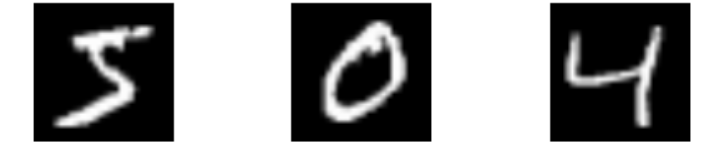
\includegraphics[width=1\linewidth]{mnist_sample}
  \captionof{figure}{Three sample images from the MNIST dataset.}
  \label{fig:test1}
\end{minipage}%
\begin{minipage}{.5\textwidth}
  \centering
  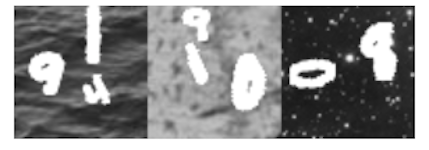
\includegraphics[width=1\linewidth]{emnist_sample}
  \captionof{figure}{Three sample images from the EMNIST dataset.}
  \label{fig:test2}
\end{minipage}
\end{figure*}

In this project, we address the digit classification task on a more difficult dataset called Extended-MNIST (EMNIST). Each example in the EMNIST dataset was generated with the following procedure:
\begin{enumerate}
\item Randomly select 2 or 3 images from MNSIT.
\item Rescale each image by a factor ranging from 40\% to 120\% the original size (the label of the generated image is that of the MNIST image which was scaled up by the largest factor).
\item Apply random rotations to each image. 
\item Superimpose these rotated images onto a random background.
\end{enumerate}

The inherent randomness in the EMNIST examples makes image classification on EMNIST more difficult than on MNIST [Figure 2]. 

In this report, we discuss the pre-processing measures we took to address the noisy features of the EMNIST examples. We then summarize our process of fitting and tuning Logistic Regression, Feedforward Neural Network, and Convolutional Neural Network (CNN) classifiers. CNNs proved most effective; we achieved 92.9\% validation accuracy using the aggregated predictions of four CNN models. We then summarize our results and our shortcomings, and ways in which we can improve our accuracy in the future. 

\section{Feature Design}

The EMNIST dataset introduces several difficulties in building an effective classifier. The random backgrounds of each example in the EMNIST dataset were generated independently of the examples' labels. Thus, they only add noise to each image, which can impede effective learning by a machine learning algorithm. 

It is also unclear which digit in each image was scaled up the most during the construction of each example in EMNIST, as we do not have prior knowledge of the dimensions of the digits used to create each example. This makes it difficult to isolate the digit within each EMNIST example that corresponds with the target label.

Finally, an effective classifier for the EMNIST dataset must be robust to rotated images, as the EMNIST dataset was built by rotating MNIST images randomly. Most machine learning algorithms are insensitive to rotations in input data, this adds much difficulty to the classification task.

\subsection{Removing Noisy Backgrounds} 

The first preprocessing step we took was to remove the backgrounds of each example in EMNIST. Luckily, the pixels in each example corresponding to the handwritten digits have a fully saturated grayscale value (corresponding to the color white). This made it possible to replace the random backgrounds with black backgrounds, by converting all non-white pixels to black pixel values [Figure 3].
\begin{figure}[H]
      \centering
      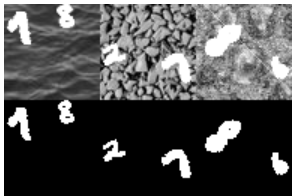
\includegraphics[scale = 1]{blackout}
		\centering
      %\includegraphics[scale=1.0]{figurefile}
      \caption{Three sample images from EMNIST, before filling the backgrounds (top) and after filling the backgrounds (bottom).}
      \label{figurelabel}
   \end{figure}

\subsection{Extracting the 'Largest' Digit} 

Each example in EMNIST contains several digits, but only one label. Intuitively, this makes the learning task difficult, as a machine learning algorithm will try associate the properties of all the  digits in an example with the example's label, when the task is to only correctly identify the \emph{largest} digit. 

Thus, we set out to extract the \emph{"largest"} digit from each example in EMNIST. Since we do not know the original dimensions of each of the digits in each image, we employed a series of heuristics to define the size of a digit. These heuristics are:
\begin{enumerate}
\item \textbf{Bounding Rectangle Area:} The area of the smallest upright rectangle that circumscribes the digit. 
\item \textbf{Bounding Circle Area:} The area of the smallest circle which circumscribes the digit. 
\item \textbf{Minimum Rotated Rectangle Area:} The area of the smallest (possibly rotated) rectangle that escribes the digit.
\item \textbf{Minimum Rotated Rectangle Maximum Dimension} The largest dimension (height,width) of the smallest (possibly rotated) rectangle that circumscribes the digit. 
\end{enumerate}
We refer to these huristics as \emph{heuristics 1-4}, respectively.

\begin{figure}[H]
      \centering
      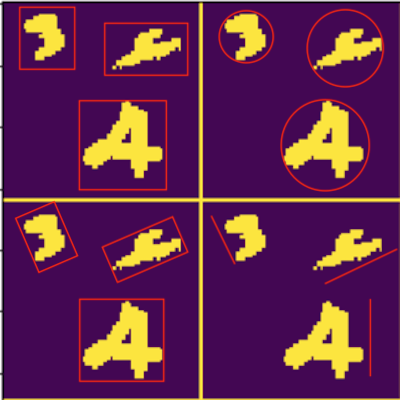
\includegraphics[scale = 1]{size_definitions}
		\centering
      %\includegraphics[scale=1.0]{figurefile}
      \caption{A sample image from EMNIST, superimposed by the geometric objects used to measure the size of each image using heuristics 1-4. Heuristic 1 is the top left, Huerustic 2 is the top right, Heuristic 3 is the bottom left, and Heuristic 4 is the bottom right.}
      \label{figurelabel}
   \end{figure}

Each heuristic defines a different definition of the size of a digit, and thus may identify a different digit to be the "largest." For each heuristic, we created a processed dataset where the largest digit was extracted from each example, according to that heuristic's size definition. We treated the choice of heuristic as a hyperparameter, and selected which heuristic to use based on which heuristic yields the highest validation accuracy for each model.

Finally, for all the datasets where one digit was extracted, we centered each image over a 28x28 pixel black square, resizing the original image as necessary while preserving the original aspect ratio. We then added a thin black border to each image, and normalized all pixel values so that they take on the values zero or one\footnote{zero corresponding to black pixels, white corresponding to white pixels}. 

\subsection{Data Augmentation} 

To help make our model more robust to rotated digits, we augmented our training data with randomly rotated copies of each training example. We tuned the number of times we rotated each image (called the \emph{"Batch Size"}), and the range of degrees with which we rotated each image as hyperparameters. 

\begin{figure}[H]
      \centering
      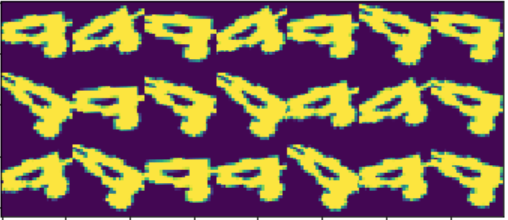
\includegraphics[scale = 1]{rotated_nines}
		\centering
      %\includegraphics[scale=1.0]{figurefile}
      \caption{A sample digit extracted from an EMNIST example after data augmentation. The original image yields a batch size of 21, with random rotations in the range [-20, 20].}
      \label{figurelabel}
   \end{figure}


\section{ALGORITHMS}

We trained classifiers of three types: Regularized Logistic Regression, Feedforward Neural Network (FFNN), and Convolutional Neural Networks (CNN). We trained each of these classifiers on the datasets processed using each of size heuristics described above, though we only experimented with data augmentation when training CNNs.

Regularized Logistic regression served as our benchmark, as it is a simple and easily implemented algorithm. 

For all experiments using FFNNs, we learned the parameters using Stochastic Gradient Descent (SGD). We used the sigmoid activation function for all hidden units and the output units, and took a model's predictions for example $X_i$ to be the class which has the highest output activation:
$$
\hat{y_i} = \argmax_{\text{Output Units; } a_i}{\sigma(a_i)}
$$
Where $\sigma$ is the logistic sigmoid function. Thus, the loss function we used was the multi-class log-loss, which is defined for a $k$ class classification problem as:
$$
Loss(\hat{y}_i, y_i) = -1\sum_{k = 1}^K*\big( y_{i,k}\log(\hat{y}_{i,k}) + (1 - y_{i,k})\log(1 - \hat{y}_{i,k}))
$$
Where $y_{i} \in \mathbb{R}^k$ is a one-hot representation of the $i^{th}$ output, and $\hat{y}_{i,k}$ is the predicted probability that example $i$ belongs in class $k$. 

Finally, we trained CNNs of four different architectures - all inspired by the LeNet architecture (Lecun et. al; 1995). These architectures alternate between convolutional and max-pooling layers, and output predictions through two fully connected layers. Of the four architectures we experimented with, one had three convolutional layers, two had four convolutional layers, and one had six convolutional layers. A summary of the four architechtures we experimented with is presented in the appendix. We refer to them as \emph{Architecture 1-4}. 
\begin{figure}[H]
      \centering
      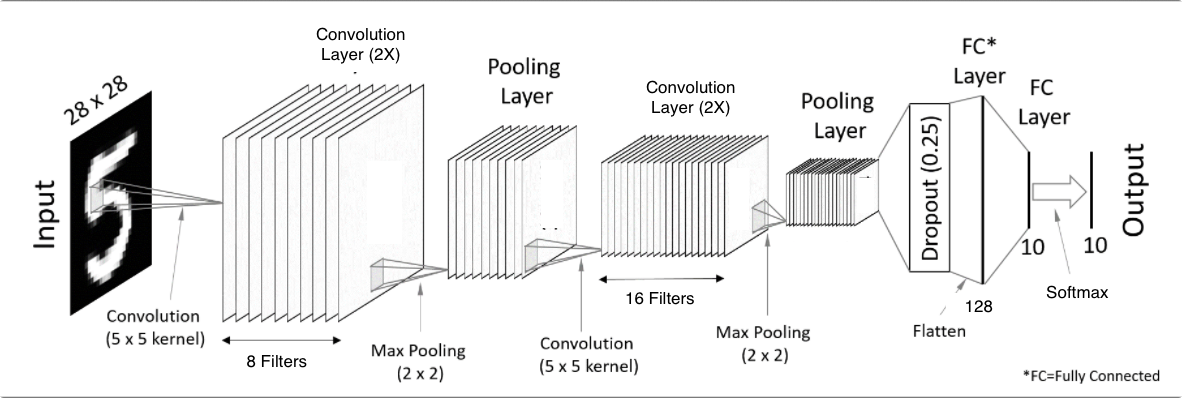
\includegraphics[scale = .42]{conv4_arch}
		\centering
      %\includegraphics[scale=1.0]{figurefile}
      \caption{One of the four CNN architectures we experimented with. The other three differ slightly in the kernel sizes, pooling sizes, and number of convolutional layers. Image modified from [6].}
      \label{figurelabel}
\end{figure}

\section{METHODOLOGY}

We started by splitting the labeled data into training and validation splits of sizes 40,000 and 10,000 examples, respectively. We kept these splits consistent in all experiments, so that we could gauge the relative effectiveness our different models. For each of the three algorithms we used, we chose which size heuristic(s) to use based on which heuristic(s) yielded the highest validation accuracy when used to select the largest digit during preprocessing. We also used this validation set to tune model-specific parameters.

\subsection{Regularized Logistic Regression: Model Hyperparameters} 

The two hyperparamters we tuned the for logistic regression were the inverse-regularization coefficient, $C$\footnote{In the notation seen in class, $C \propto \sfrac{1}{\lambda}$.}, and the regularization loss function (either \emph{l1} or \emph{l2}). Using the processed datasets generated from using each of the four size heuristics, we ran a grid-search over 24 hyperparameter combinations, and selected the combination that yielded the best validation accuracy.   

\subsection{Feedforward Neural Network: Model Hyperparameters} 

The two hyperparameters we tuned when using FFNNs were the learning rate, $\eta$, and the model architecture. We did not implement regularization.

\subsection{Feedforward Neural Network: Learning Optimizations} 

We began by trying to fit our models using simple SGD, but quickly found that our models were not converging. 

To address this, we implemented \emph{momentum} to help calculate the ammount each weight $\theta$ should be updated on iteration $t$, denoted $\nu_t$, where $\nu_t$ is defined:
$$
\nu_t = \gamma\nu_{t-1} - \eta\nabla_{\theta}\text{Loss}(\theta)
$$
Where $\gamma$ is an additional hyperparameter introduced. 

We also implemented \emph{power scaling} - a method of slowly reducing the learning rate $\eta$ with each epoch. At the end of each epoch, $\eta$ is updated as follows:
$$
\eta_{\text{new}} = \frac{\eta_{\text{old}}}{(\text{Epoch number})^{p}}
$$
for a scaling parameter $p$. This allows the weights to change drastically in the begining of training, and slowly dampens the change in weights as training progresses, so that local maxima are not overlooked. 

We found that introducing these two learning optimizations helped the SGD algorithm minimize loss much faster. Thus, for all experiments with FFNN, we used both momentum and power scaling, with the hyperparameters fixed at $\gamma = .9, p = .9$. 

\subsection{Convolutional Neural Network: Hyperparameter Tuning} 

We considered many hyperparameters when tuning our CNN models. The most important hyperparameters are summarized in Table 1.
\begin{table}[b]
\caption{Hyperparameter Ranges Explored for CNN models}
\centering
\label{my-label}
\begin{tabular}{|c|c|}
\hline
\textbf{Hyperparameter}                                                                     & \textbf{Range Explored}                                                                                                            \\ \hline
Model Architecture                                                                          & \begin{tabular}[c]{@{}c@{}}\{Architecture 1, Architecture 2, \\ Architecture 3, Architecture 4\}\end{tabular}                      \\ \hline
\begin{tabular}[c]{@{}c@{}}Data Augmentation - \\ (Batch size, Rotation Range)\end{tabular} & \begin{tabular}[c]{@{}c@{}}\{(1, {[}0, 0{]}), \\ (8, {[}-10, 10{]}), \\ (16, {[}-20, 20{]}), \\ (16, {[}-30, 30{]})\}\end{tabular} \\ \hline
\multicolumn{1}{|l|}{Learning Rate}                                                         & \multicolumn{1}{l|}{\{.00001, .00005, .0001\}}                                                                                  \\ \hline
Digit Size Heuristic                                                                        & \begin{tabular}[c]{@{}c@{}}\{Heuristic 1, Heuristic 2,\\  Heuristic 3, Heuristic 4\}\end{tabular}                                  \\ \hline
\end{tabular}
\end{table}

We started by training all four architectures on the data preprocessed using Heuristic 1 with the high learning rate of $.0001$. After observing that architectures 2 and 4 yielded much higher validation accuracy than architectures 1 and 3, we decided to omit the latter architectures from all further experiments.

We then took a random sample of 64 images from EMNIST, and extracted the "largest" digit from each image using each of the four size heuristics defined. We observed by visual inspection that when using Heuristics 2 and 4, we isolated the digits corresponding to the labels more frequently than when we used Heuristics 1 and 3. We decided to use data preprocessed with Heuristics 2 and 4 in all further experiments. 

We then performed a gridsearch on the remaining hyperparameter combinations permitted by the constrained hyperparameter ranges [Table 2], totaling 32 hyperparamter combinations.


\begin{table}[]
\centering
\caption{Constrained Hyperparameter Ranges}
\label{my-label}
\begin{tabular}{|c|c|}
\hline
\textbf{Hyperparameter}                                                                     & \textbf{Range Explored}                                                                                                            \\ \hline
Model Architecture                                                                          & \{Architecture 2, Architecture 4\}                                                                                                 \\ \hline
\begin{tabular}[c]{@{}c@{}}Data Augmentation - \\ (Batch size, Rotation Range)\end{tabular} & \begin{tabular}[c]{@{}c@{}}\{(1, {[}0, 0{]}), \\ (8, {[}-10, 10{]}), \\ (16, {[}-20, 20{]}), \\ (16, {[}-30, 30{]})\}\end{tabular} \\ \hline
Learning Rate                                                                               & \{.00001, .00005\}                                                                                                               \\ \hline
Digit Size Heuristic                                                                        & \{Heuristic 2, Heuristic 4\}                                                                                                       \\ \hline
\end{tabular}
\end{table}


\subsection{CNN: Learning Optimization} 

We learned the weights of our networks using the \emph{RMSProp} algorithm, with the hyperparameter $\rho$ fixed at 0.9. While learning, we used an early stopping scheme, which caused training to stop if the validation accuracy has not improved for 8 consecutive epochs. 

At first, we tried learning using learning rate of $\eta = .0001$, but we observed through the use of learning curves that the convergence had very high variance. After reducing the learning rate to $.00005$, we achieved smoother learning [Figure 7]. Thus, we limited the range of values or $\eta$ to consider to $\eta \in \{.00005, .00001\}$.

\begin{figure}
      \centering
      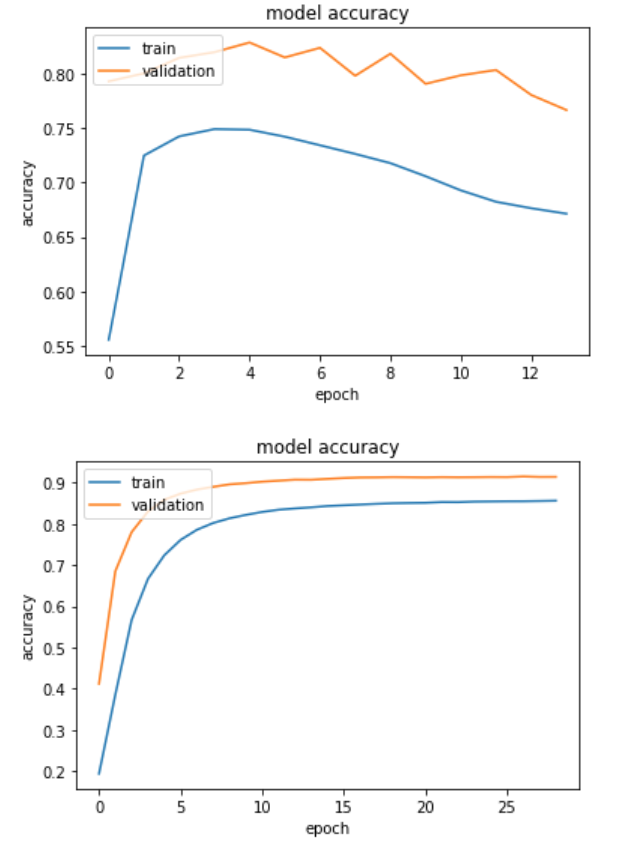
\includegraphics[scale = .6]{learning_curves.png}
		\centering
      %\includegraphics[scale=1.0]{figurefile}
      \caption{Learning curves for training periods with $\eta = .0001$ and $\eta = .00005$, with early stopping. Note: training accuracy is lower than validation accuracy. This is because we used data augmentation, and the new randomly rotated images made the training data "harder" to learn than the validation data.}
      \label{figurelabel}
\end{figure}

\subsection{CNN: Aggregated Predictions} 

We initialized the weights of our CNN's randomly. As such, every time we fit a CNN with fixed configuration, the final weights were not guaranteed to be the same, potentially leading to different predictions. 

To account for this randomness, we fit two models of each hyperparameter configuration, each with different random initialization. This allowed us to keep the better of the two trained models (based on validation-set accuracy) for each hyperparameter configuration. Further, this presented us with the opportunity to aggregate the predictions of our best performing CNN configurations\footnote{To aggregate predictions of several models, we used the class which was predicted the most frequently amongst all models to be the aggregated class prediction.}.

We experimented with the aggregations of the predictions of our four best CNN models, in terms of validation accuracy. We refer to these CNN configurations as \emph{CNN 1-4}. 

Two of these aggregations increased validation accuracy by over 1\%. We refer to these aggregations as \emph{Aggregation 1} and \emph{Aggregation 2}. 

\textbf{Aggregation 1:}
\begin{itemize}
\item Predictions of four models aggregated.
\item All four top CNN configurations used exactly once:
	\begin{itemize}
    \item CNN 1: Architechture 2, Batch Bize = 16, Rotation Range [-.2, .2], $\eta$ = .00005, Size Heuristic 2
	\item CNN 2: Architechture 4, Batch Bize = 16, Rotation Range [-.2, .2], $\eta$ = .00005, Size Heuristic 2
	\item CNN 3: Architechture 2, Batch Bize = 16, Rotation Range [-.2, .2], $\eta$ = .00005, Size Heuristic 4
	\item CNN 4: Architechture 4, Batch Bize = 16, Rotation Range [-.2, .2], $\eta$ = .00005, Size Heuristic 4
	\end{itemize}
\end{itemize}
\textbf{Aggregation 2:}
\begin{itemize}
\item Predictions of four models aggregated.
\item CNN 1 and CNN 2 were both trained twice with different intitializations, and included in the aggregation twice.
\end{itemize}

\section{RESULTS}

In this section we discuss the hyperparameters which had the largest impact on the performance of each model, and then we compare the perforance of each of our tuned models on the validation set. 

\subsection{Regularized Logistic Regression} 

After doing a thorough search through many $\big(\text{C}, \text{Regularization Loss Function}\big)$ combinations, we found that the hyperparameter which had the largest impact on validation accuracy was the regularization loss function. The best model trained with $l1$-loss achieved a validation accuracy over 1\% higher than the best model trained with $l2$-loss [Table 3].

\begin{table}[H]
\centering
\caption{Best Logistic Regression Models, Trained with l1/l2 Loss}
\label{my-}
\begin{tabular}{|c|c|c|}
\hline
\textbf{Loss Function} & \textbf{Regularization Parameter} & \textbf{Validation Accuracy} \\ \hline
l1-loss                & 0.09                              & 0.731                        \\ \hline
l1-loss                & .27                               & \textbf{0.735}               \\ \hline
l2-loss                & .01                               & 0.723                        \\ \hline
l2-loss                & .03                               & 0.721                        \\ \hline
\end{tabular}
\end{table}

Models trained with $l1$-loss regularization find sparse solutions - meaning that many input features do not contribute to the decision boundary. This has an interesting interpretation for the EMNIST classification problem; it means that the Logistic Regression model learned that some pixel values (features) do not help to predict the largest digit, and should be ignored.

For example, since we padded all images with a black border during preprocessing, these pixel values do not help to distinguish between the digits. Its reasonable to assume that the Logistic Regression model, trained with $l1$-loss learned to ignore the values of those pixels.

\subsection{Feedforward Neural Network} 

We experimented with three model architectures when fitting our FFNN:

\begin{table}[H]
\centering
\caption{FFNN Architectures}
\label{my-label}
\begin{tabular}{|c|c|c|}
\hline
\textbf{\begin{tabular}[c]{@{}c@{}}Architecture\\ Number\end{tabular}} & \textbf{\begin{tabular}[c]{@{}c@{}}Number of\\ Hidden Layers\end{tabular}} & \textbf{\begin{tabular}[c]{@{}c@{}}Hidden Layer\\ Dimensions\end{tabular}} \\ \hline
Architecture 1                                                         & 1                                                                          & (128)                                                                      \\ \hline
Architecture 2                                                         & 2                                                                          & (64, 20)                                                                   \\ \hline
Architecture 3                                                         & 2                                                                          & (128, 64)                                                                  \\ \hline
\end{tabular}
\end{table}

We trained all models for 20 epochs with SGD, using both momentum and power scaling. 

After some experimentations, we found that the configuration $\eta = .01, \gamma = .9, p = .9$ led to a reasonable convergence rate. Using these hyperparameter configurations, we fit each of the architectures described in table 3, and got the following results:

\begin{table}[H]
\centering
\caption{Validation Accuracies for FFNN Experiments}
\label{my-label}
\begin{tabular}{|c|c|}
\hline
\textbf{\begin{tabular}[c]{@{}c@{}}Architecture\\ Number\end{tabular}} & \textbf{\begin{tabular}[c]{@{}c@{}}Validation \\ Accuracy\end{tabular}} \\ \hline
Architecture 1                                                         & .55                                                                     \\ \hline
Architecture 2                                                         & .64                                                                     \\ \hline
Architecture 3                                                         & .64                                                                     \\ \hline
\end{tabular}
\end{table}

Of the three architectures we used, those with two hidden layers achieved almost 10\% better accuracy on the validation set. We have not tuned these models thoroughly, however, and so we cannot yet conclude that FFNNs with two hidden layers perform better on the EMNIST classification task than those with one hidden layer. Perhaps with more training, changes to the number of hidden units, and tuning to the learning hyperparameters $\gamma$ and $p$, a FFNN with one hidden unit could outperform Architectures 2 and 3. 

\subsection{Convolutional Neural Network} 

When training our CNNs, the performance of our models was not very sensitive to the learning rate $\eta$. In fact, we saw no evidence that models trained with the learning rate $\eta = .00001$ yielded higher validation accuracy than models trained with $\eta = .00005$ - all else fixed. 

A hyperparameter which had a noticeable effect was the choice of data augmentation scheme. Our best model trained without data augmentation yielded validation accuracy almost 2\% lower than our best model trained with data augmentation. 

We found that the benefits of data augmentation diminished as we increased the rotation range past $[-20,20]$. One explanation for this is that if one distorts the training data too severely, it makes the learning problem \emph{"too hard"}, and a classifier has trouble picking up on patterns in the modified training data. 

Thus, we found that the best configuration for data augmentation was a Batch Size of 16, with rotation range $[-20,20]$ [table 6].

% Please add the following required packages to your document preamble:
% \usepackage[table,xcdraw]{xcolor}
% If you use beamer only pass "xcolor=table" option, i.e. \documentclass[xcolor=table]{beamer}
\begin{table}[]
\centering
\caption{Best CNN Models for Different Data Augmentation Schemes}
\label{my-label}
\begin{tabular}{|c|c|
>{\columncolor[HTML]{ECF4FF}}c |
>{\columncolor[HTML]{ECF4FF}}c |
>{\columncolor[HTML]{ECF4FF}}c |}
\hline
\textbf{\begin{tabular}[c]{@{}c@{}}CNN\\ Architecture\end{tabular}} & \textbf{\begin{tabular}[c]{@{}c@{}}Digit Size\\ Heuristic\end{tabular}} & \textbf{\begin{tabular}[c]{@{}c@{}}Batch\\ Size\end{tabular}} & \textbf{\begin{tabular}[c]{@{}c@{}}Rotation\\ Range\end{tabular}} & \textbf{\begin{tabular}[c]{@{}c@{}}Validation\\ Accuracy\end{tabular}} \\ \hline
4                                                                   & 2                                                                       & 1                                                             & -                                                                 & 89.4                                                                   \\ \hline
4                                                                   & 2                                                                       & 16                                                            & {[}-20, 20{]}                                                     & \textbf{91.2}                                                          \\ \hline
4                                                                   & 2                                                                       & 16                                                            & {[}-30, 30{]}                                                     & 90.3                                                                   \\ \hline
\end{tabular}
\end{table}

We also found that aggregating predictions of serveral models led to an increase in validation accuracy.

The four CNN configurations which achieved the best validation accuracy are specified in section \emph{4.f}, and are referred to as \emph{CNN 1-4}. The predictions of these models were pooled to create Aggregation 1. The pooled predictions of Aggregation 1 achieved better validation accuracy than any of the individual models used to construct it. Further, we found that Aggregation 2 yielded the best validation accuracy [Table 7]. 

\begin{table}[b]
\centering
\caption{Highest performing CNN Models and Aggregations}
\label{my-label}
\begin{tabular}{|c|c|}
\hline
\textbf{\begin{tabular}[c]{@{}c@{}}CNN \\ Configuration\end{tabular}} & \textbf{\begin{tabular}[c]{@{}c@{}}Validation \\ Accuracy\end{tabular}} \\ \hline
CNN 1                                                                 & .910                                                                    \\ \hline
CNN 2                                                                 & .918                                                                    \\ \hline
CNN 3                                                                 & .906                                                                    \\ \hline
CNN 4                                                                 & .911                                                                    \\ \hline
\end{tabular}
\begin{tabular}{|l|l|}
\hline
\textbf{Aggregation} & \textbf{\begin{tabular}[c]{@{}l@{}}Validation \\ Accuracy\end{tabular}} \\ \hline
Aggregation 1        & .921                                                                    \\ \hline
Aggregation 2        & \textit{\textbf{.929}}                                                  \\ \hline
\end{tabular}
Validation accuracies of best four CNN configurations, and those of aggregated predictions. Aggregation 1 was created by pooling the predicions of CNN 1-4 once, and Aggregation 2 was created by pooling the predictions of CNN 1 and 2 twice - after training both configurations twice with different initializations.
\end{table}

This may suggest that the errors which of each of the models that we pooled "canceled out," simulating the predictions of a classifier with lower variance and increased prediction performance. Furthermore, due to the fact that all four models used to construct Aggregation 2 were trained on data preprocessed using Size Heuristic 2 - and that the predictions of Aggregation 2 led to the highest validation accuracy we achieved - we are inclined to believe that Heuristic 2 does the best job of identifying the "largest" digit in each image amongst the heuristics we proposed. 

Overall, our CNN models had the performed the best out of all our models; our final predictions were those of Aggregation 2 - with a validation accuracy of 92.9\% and a public leaderboard accuracy of 93.0\%. This validates our initial hypothesis that CNNs are an appropriate model class for the EMNIST classification problem.

\section{DISCUSSION AND CONCLUSIONS}

After running our experiments, we have concluded that CNNs achieve the best performance out of the three model classes that we trained. However, due to performance issues, we did not tune the hyperparameters of our FFNNs thoroughly enough to conclude that FFNN cannot achieve competitive performance. We would likely benefit from tuning our model architectures, and allowing our networks to train for more epochs. 

Furthermore our FFNN implmentation was very simplistic. Some of the optimizations we could implement that would likely help performance are:

\begin{itemize}
\item Regularization, and tune regularization parameter. We could also try to limit overfitting by implementing dropout.
\item Experiment with more learning methods (besides SGD), such as Batch Gradient Descent, and more advanced update rules, such as RMSProp or ADAM.
\item Backpropogation optimizations, such as Batch Normalization.  
\end{itemize}

Although we meticulously tuned the hyperparameters associated with our CNN models, we only considered a limited scope of model architectures. All four architectures we experimented with were variants of the LeNet architecture. 

Although LeNet has proved effective in classifying handwritten digits by many authors, we would like to experiment with a more diverse range of architectures in the future. One particularly exciting recent development in deep learning are Capsule Networks, proposed by Hinton et al. (2017), which may be more robust to changes in image orientation and overlapping images than CNNs - and thus applicable to this problem. 

Finally, we would like to invest more effort in improving our preprocessing methods. After visual inspection of 100 misclassified validation examples, we noticed that many of the digits that we extracted from these examples did not correspond to the correct label - meaning that we failed to extract the "largest" digit during preprocessing. We believe that our preprocessing is the bottleneck hindering us from building a more successful classifier, and that if we were to improve our preprocessing methods substantially then we could produce a more competitive solution. 

\section{Statement of Contributions}

Tamir performed the preprocessing described, built and tuned the CNN and Logistic Regression models, contributed to the FFNN implementation, and wrote this report. Kyle and Phillip contributed to FFNN implementation, as well as this report.

\addtolength{\textheight}{-12cm}   % This command serves to balance the column lengths
                                  % on the last page of the document manually. It shortens
                                  % the textheight of the last page by a suitable amount.
                                  % This command does not take effect until the next page
                                  % so it should come on the page before the last. Make
                                  % sure that you do not shorten the textheight too much.

%%%%%%%%%%%%%%%%%%%%%%%%%%%%%%%%%%%%%%%%%%%%%%%%%%%%%%%%%%%%%%%%%%%%%%%%%%%%%%%%



%%%%%%%%%%%%%%%%%%%%%%%%%%%%%%%%%%%%%%%%%%%%%%%%%%%%%%%%%%%%%%%%%%%%%%%%%%%%%%%%



%%%%%%%%%%%%%%%%%%%%%%%%%%%%%%%%%%%%%%%%%%%%%%%%%%%%%%%%%%%%%%%%%%%%%%%%%%%%%%%%


\newpage
\begin{thebibliography}{99}
\bibitem{c1} Cohen, G., Afshar, S., Tapson, J., \& van Schaik, A. (2017). EMNIST: an extension of MNIST to handwritten letters. Retrieved from http://arxiv.org/abs/1702.05373 (link is external)
\bibitem{c2} Y. LeCun, L. Bottou, Y. Bengio and P. Haffner: Gradient-Based Learning Applied to Document Recognition, Intelligent Signal Processing, 306-351, IEEE Press, 2001,
\bibitem{c3} Y. LeCun, L. D. Jackel, L. Bottou, A. Brunot, C. Cortes, J. S. Denker, H. Drucker, I. Guyon, U. A. Muller, E. Sackinger, P. Simard and V. Vapnik: Comparison of learning algorithms for handwritten digit recognition, in Fogelman, F. and Gallinari, P. (Eds), International Conference on Artificial Neural Networks, 53-60, EC2 \& Cie, Paris, 1995.
\bibitem{c4} Pedregosa et al. Scikit-learn: Machine Learning in Python, JMLR 12, pp. 2825-2830, 2011
\bibitem{c5} G.Hinton, S.Sabour and N. Frosst: Dynamic Routing Between Capsules. CoRR, 2017. Retrieved from http://arxiv.org/abs/1710.09829
\section*{Blog Posts}

\bibitem{c6} Theart, R. (2017, November 29). Getting started with PyTorch for Deep Learning (Part 3: Neural Network basics). Retrieved from https://codetolight.wordpress.com/2017/11/29/getting-started-with-pytorch-for-deep-learning-part-3-neural-network-basics/


\end{thebibliography}

\newpage
\section{APPENDIX}
\begin{figure}[H]
      \centering
      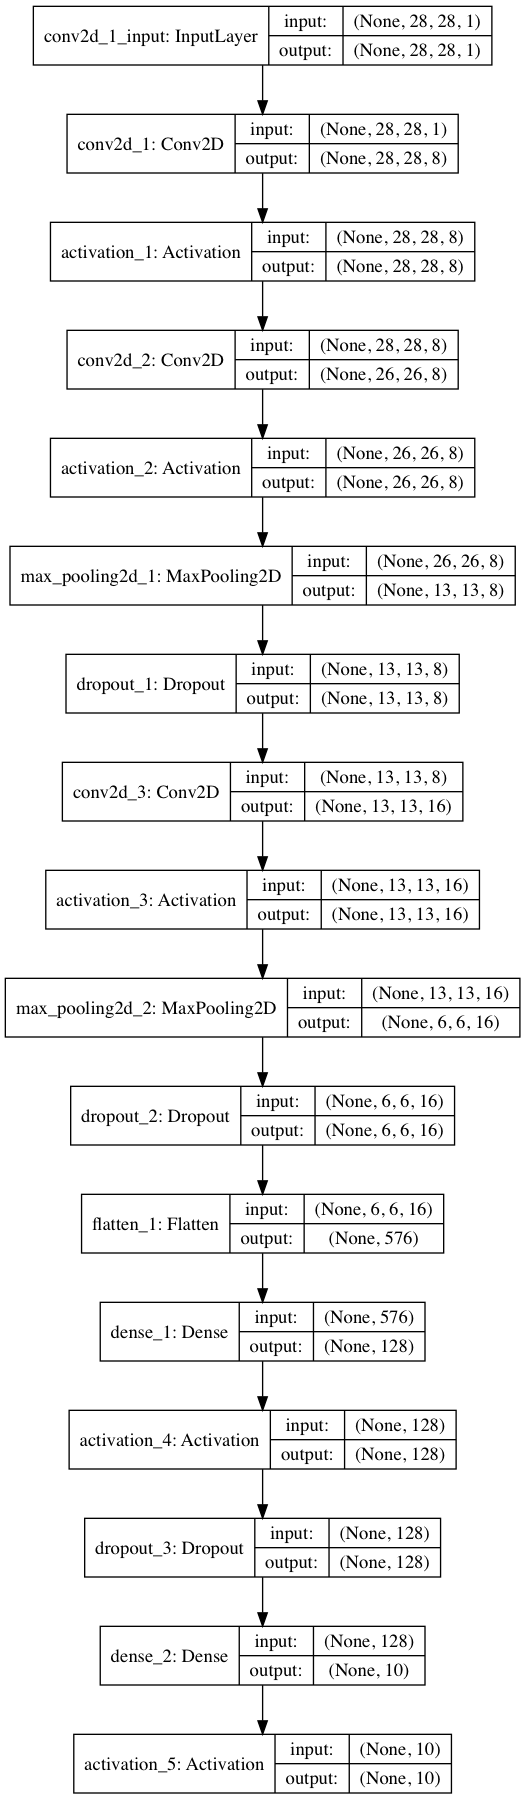
\includegraphics[scale = .35]{model0.png}
		\centering
      %\includegraphics[scale=1.0]{figurefile}
      \caption{Architecture 1: Three convolutional layers, 76,978 trainable parameters.}
      \label{figurelabel}
   \end{figure}
   
\begin{figure}[H]
      \centering
      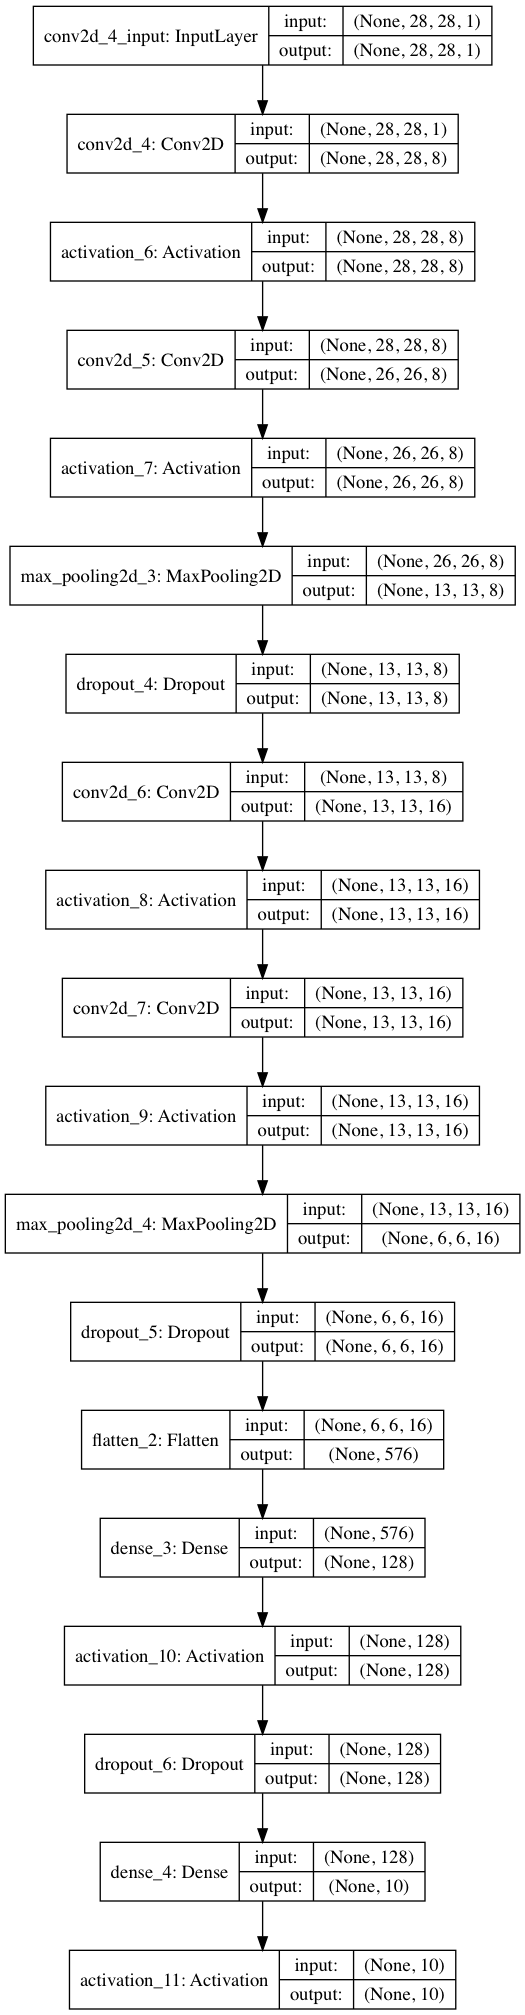
\includegraphics[scale = .3]{model1.png}
		\centering
      %\includegraphics[scale=1.0]{figurefile}
      \caption{Architecture 2: Four convolutional layers, 79,298 trainable parameters.}
      \label{figurelabel}
   \end{figure}
   
\begin{figure}[H]
      \centering
      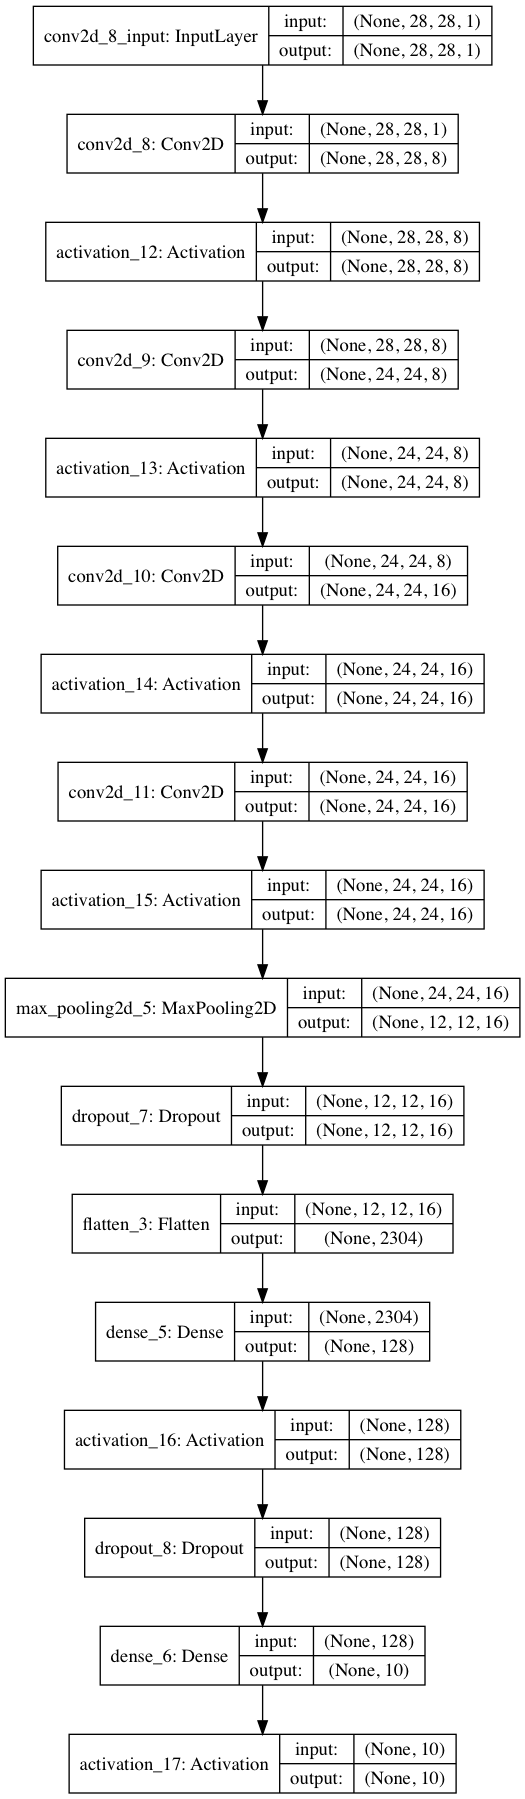
\includegraphics[scale = .3]{model2.png}
		\centering
      %\includegraphics[scale=1.0]{figurefile}
      \caption{Architecture 3: Four convolutional layers, 307,778 trainable parameters.}
      \label{figurelabel}
   \end{figure}
   
\begin{figure}[H]
      \centering
      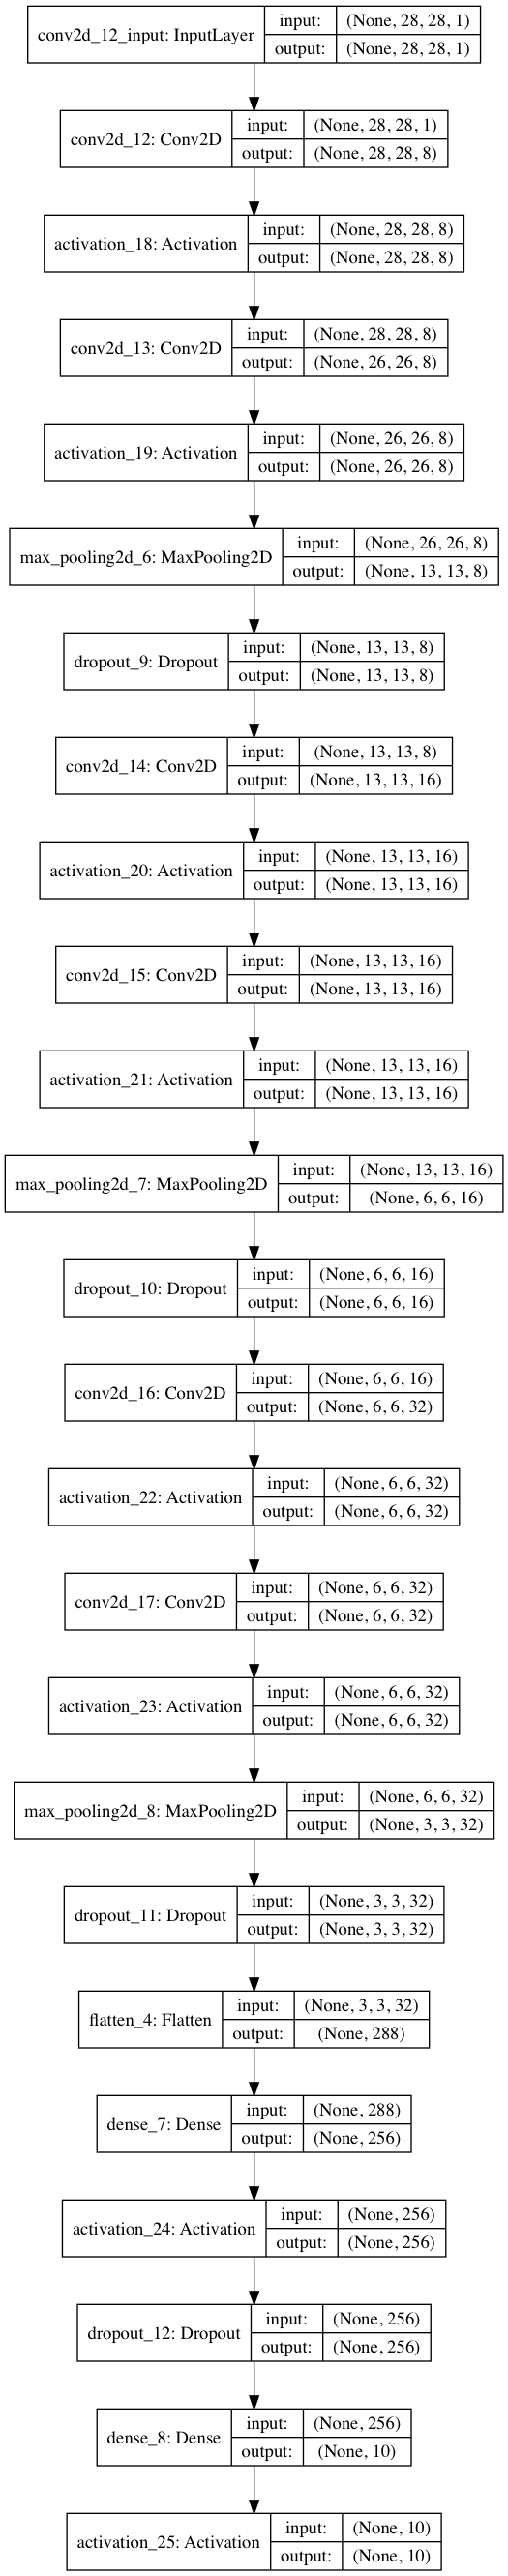
\includegraphics[scale =.2]{model3.png}
		\centering
      %\includegraphics[scale=1.0]{figurefile}
      \caption{Architecture 4: Six convolutional layers, 94,594 trainable parameters.}
      \label{figurelabel}
 \end{figure}




\end{document}
